\documentclass[11pt]{article}

% ACL camera-ready style.  The local acl.sty and acl_natbib.bst files are copied
% from https://github.com/acl-org/acl-style-files/.
\usepackage{acl}

\usepackage{times}
\usepackage{latexsym}
\usepackage[T1]{fontenc}
\usepackage[utf8]{inputenc}
\usepackage{microtype}
\usepackage{amsmath}
\usepackage{booktabs}
\usepackage{graphicx}
\usepackage{placeins}

\setlength{\textfloatsep}{8pt plus 2pt minus 2pt}
\setlength{\floatsep}{7pt plus 2pt minus 2pt}
\setlength{\intextsep}{7pt plus 2pt minus 2pt}
\setlength{\abovecaptionskip}{4pt}
\setlength{\belowcaptionskip}{0pt}

\newcommand{\LabelSupports}{\mbox{\textsc{Supports}}}
\newcommand{\LabelRefutes}{\mbox{\textsc{Refutes}}}
\newcommand{\LabelNEI}{\mbox{\textsc{NEI}}}
\newcommand{\LabelDisputed}{\mbox{\textsc{Disputed}}}

\title{AI Fact-Checking System}

\author{
  Group\_131 \\
  COMP90042 Project 2026
}

\begin{document}
\raggedbottom
\maketitle

\begin{abstract}
We demonstrate an efficient resource-optimized pipeline involving fact-checking 
for the climate-based claims executing in the free-tier of the Google Colab kernel 
runtime avoids any additional services, checkpoints of saved models, or already 
computed indexes. The system represents the issues of verdict predictions and 
retrieval of evidence below a constrained budget of compute via four staged parts: 
One multi-gate sparse retriever which applies a appropriately weighted reciprocal 
rank fusion over the views of BM25; the multi-scaling feature fusion reranker 
integrates similarity of sentence embedding and the shallow factual alignment cues 
involving numeric agreement, lexical overlapping, and the compatibility with the 
negation; the bounded cross-encoder selector only used on a candidate subset which
is prefiltered; and TF-IDF which is a structured-organized logistic classifier which
encodes the factual cue tokens and the rank of evidence as input signals that are
explicit. In this respective development set, our best Colab-supporting configuration 
attains a solid evidence retrieval score of 0.2021, claim classification accuracy of 
0.5000, harmonic mean of 0.2879, and the classifier macro-F1 score of 0.4659. The 
point to be noted is that we must safeguard the shallow factual cues and the evidence 
rank on the way via the pipeline, instead of throwing them through the concatenation
of plain evidence, which uniformly enhances the performance of the classifier.
\end{abstract}

\section{Introduction}

Climate-related claims usually appear as short statements in news articles,
social media posts, or public discussions, while the information needed to
verify them is often scattered across a much larger evidence corpus. This makes
climate fact-checking different from ordinary claim classification: the model
is not only asked to assign a verdict, but must do so based on evidence that
has to be found before it can be used. At the same time, a practical system
cannot assume unlimited computation, especially in lightweight settings where
the full pipeline is expected to run in a free notebook environment such as
Google Colab. We therefore frame the project as a resource-constrained
evidence-based verification problem \citep{thorne2018fever,diggelmann2020climatefever}.
The goal is not to build the strongest possible model in isolation, but to
design a pipeline that gives a good balance between evidence recall, verdict
accuracy, and runtime cost.

% P2: Related work paragraph goes here.

Motivated by the resource-constrained setting, our system adopts a staged design
in which each module improves evidence quality under a bounded computational
budget. First, Multi-Gate Sparse Candidate Retrieval is used to build a
high-recall evidence pool: the Word gate captures direct lexical overlap
between claims and evidence, the Character gate improves robustness to
surface-form and morphological variation, the Structured gate emphasizes
claim-critical cues such as entities, numbers, and factual expressions, and the
Shared BM25 interaction provides a common sparse scoring basis across these
retrieval views \citep{robertson1994okapi}; Rank fusion then combines the gate
outputs into a broader and more stable candidate set than any single gate alone
\citep{cormack2009rrf}. Second, Multi-Scale Feature Fusion reranks the retrieved
candidates by combining semantic similarity with shallow factual signals, so
the system can benefit from MiniLM-style meaning matching while still preserving
precise cues such as lexical overlap, numerical consistency, negation, and
retrieval rank \citep{reimers2019sentence}. Third, Bounded Neural Evidence
Selection applies stronger neural scoring only to a prefiltered subset of
candidates, allowing the model to capture richer claim--evidence interactions
without applying expensive neural inference to the full corpus
\citep{nogueira2019bert}. Finally, Structured Evidence Classification converts
the selected evidence into a compact rank-aware and cue-aware representation for
verdict prediction, so the classifier uses both evidence content and retrieval
confidence while keeping the full pipeline runnable in the target low-resource
environment.

The main contribution of this work is a resource-aware evidence-based
verification pipeline that connects retrieval, reranking, evidence selection,
and verdict classification under a single executable framework. Rather than
optimizing each component in isolation, the system is designed around the
performance--runtime trade-off required by low-resource execution. Within this
pipeline, the key technical contributions are Multi-Gate Sparse Candidate
Retrieval, which improves candidate recall by combining complementary sparse
views; Multi-Scale Feature Fusion, which integrates semantic similarity with
shallow factual signals for more reliable reranking; Bounded Neural Evidence
Selection, which limits expensive neural scoring to the most promising
candidates; and Structured Evidence Classification, which represents selected
evidence in a form that preserves rank and factual cues for final prediction.
In addition, we contribute a set of diagnostic experiments that analyze the
effect of sparse gates, rank fusion, neural selection, evidence representation,
and classifier sensitivity, providing insight into which stages most strongly
affect evidence quality, label accuracy, and runtime.

\section{Method}

\subsection{Pipeline Overview}

Let $\mathcal{C}$ be claims and $\mathcal{E}$ evidence.  The output is a verdict
and a small evidence set per claim.  Since scoring all
$(c,e)\in\mathcal{C}\times\mathcal{E}$ pairs is infeasible, we use a staged
pipeline:
\[
\mathcal{E}\rightarrow \mathcal{A}(c)\rightarrow \mathcal{B}(c)
\rightarrow \mathcal{D}(c),
\]
where $\mathcal{A}(c)$ is a broad sparse pool, $\mathcal{B}(c)$ a reranked
context pool, and $\mathcal{D}(c)$ the submitted evidence.  Cheap stages maximize
recall; semantic models operate on progressively smaller pools.  The four
components are multi-gate sparse retrieval, multi-scale reranking, bounded
cross-encoder selection, and structured-evidence classification.

\begin{figure}[t]
\centering

\includegraphics[width=\linewidth]{figures/acl_staging_cost_benefit.png}
\caption{Staged pruning keeps recall while reducing pair count.  The candidate
and context pools retain most recoverable evidence by using neural scoring on
progressively smaller pools; full-corpus neural scoring would require about 186
million development pairs.}
\label{fig:staging}
\end{figure}

\begin{figure}[t]
\centering
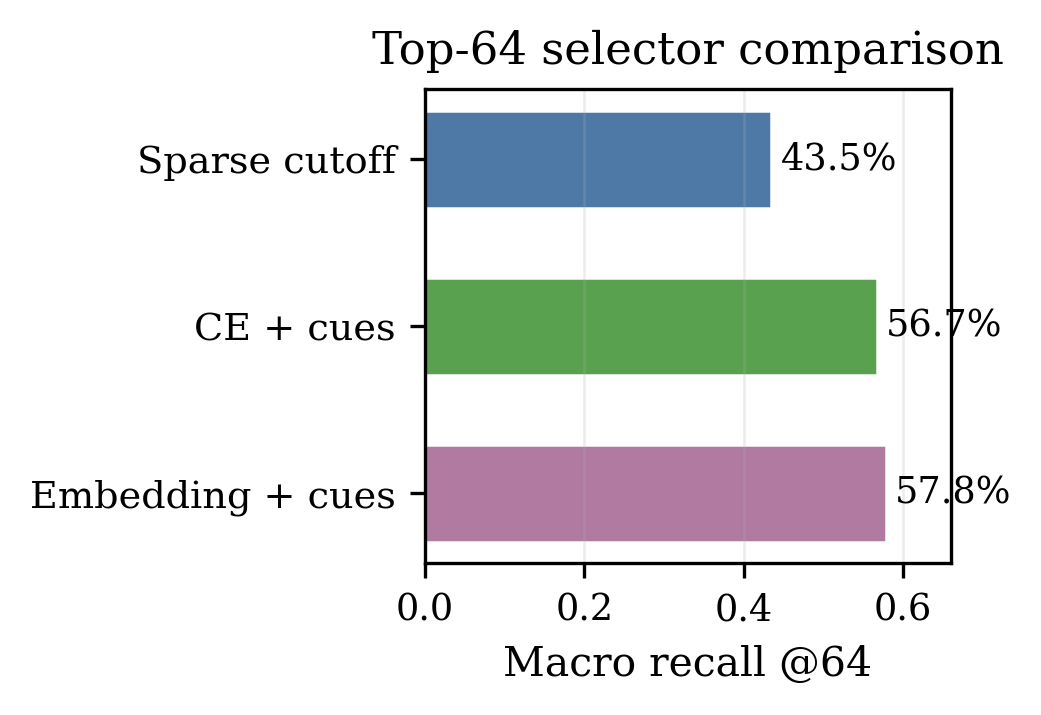
\includegraphics[width=\linewidth]{figures/acl_top64_diagnostic.png}
\caption{Embedding plus factual cues is the best top-64 selector, reaching
57.8\% macro recall above sparse cutoff and cross-encoder-plus-cue variants.}
\label{fig:top64-selector}
\end{figure}

\subsection{Multi-Gate Sparse Candidate Retrieval}

The sparse stage maximizes recall by applying one BM25 scoring operator to
multiple feature spaces \citep{robertson1994okapi}.  The four gates differ in
analyzer $a_g(\cdot)$ and vocabulary $V_g$.  Let $q_g(c)$ and $x_g(d)$ be the
resulting count vectors for claim $c$ and evidence document $d$.  For each gate,
the notebook builds a claim matrix $Q_g$ and an evidence matrix $X_g$, reweights
the evidence matrix with BM25, and computes batched sparse products
$Q_gX_g^\top$ before retaining the top-ranked evidence rows per claim.

\paragraph{Word gate.}
Word terms give the direct lexical view: content-word overlap raises scores and
IDF weighting emphasizes discriminative claim terms.  The analyzer removes
English stop words and uses both unigrams and adjacent word bigrams, so phrase
matches such as scientific terms or named processes can contribute as single
features.

\paragraph{Character gate.}
Character n-grams capture partial overlap, inflection, hyphenation, and spelling
variation missed by exact words.  This gate uses word-boundary character
n-grams, making it useful for abbreviations, compounds, and morphology in
climate terminology.

\paragraph{Structured gate.}
Structured cues keep numbers, years, salient capitalized terms, and negation
markers.  These are encoded as typed tokens such as year, number, entity-like,
and negation features, so numeric or negation agreement can affect retrieval
even when surrounding words differ.

\paragraph{Pseudo-relevance feedback gate.}
PRF expands the word query using high-ranked feedback evidence.  If
$\mathcal{F}(c)$ is the feedback set,
\[
q_{\mathrm{prf}}(c)=q_{\mathrm{word}}(c)
  + \eta\sum_{d\in\mathcal{F}(c)} w(c,d)x_{\mathrm{word}}(d),
\]
where $w(c,d)$ downweights lower-ranked feedback documents.  PRF adds related
terms absent from the original claim while staying in the sparse word space.

\paragraph{Shared BM25 interaction.}
After feature construction, each gate applies the same BM25 interaction.  For
term $t$ in document $d$,
\[
\begin{aligned}
\operatorname{idf}_t &=
\log\!\left(\frac{N-df_t+0.5}{df_t+0.5}+1\right),\\
\operatorname{BM25}_{d,t} &=
\operatorname{idf}_t
\frac{(k_1+1)f_{d,t}}
{f_{d,t}+k_1(1-b+b|d|/\overline{|d|})}.
\end{aligned}
\]
The inverse-document-frequency factor suppresses common features, so rare
claim-specific evidence terms contribute more than corpus-wide background
terms.  The query side remains a count vector, giving the sparse dot product
\[
s_g(c,d)=q_g(c)^\top \operatorname{BM25}_g(d).
\]
Thus $g$ chooses the representation, and BM25 weights it.  The notebook uses
SciPy/NumPy sparse matrices, so document-frequency counts, BM25 reweighting, and
query--document dot products run in optimized C/C++ kernels and vectorized array
operations.

\paragraph{Rank fusion.}
Each gate produces a ranked list.  The fifth sparse view is their weighted RRF
fusion \citep{cormack2009rrf}:
\[
S_{\mathrm{RRF}}(c,d)=
\sum_{g\in G}\frac{\lambda_g}{K_{\mathrm{RRF}}+r_g(c,d)},
\]
where missing documents contribute zero.  We treat $\lambda_g$ as a reliability
prior: stronger standalone gates receive larger weights, and complementary
factual gates retain smaller weights.  The structured gate contributes
complementary recall in fusion, as shown by ablation; RRF also removes the need
for cross-gate score calibration.

\begin{figure*}[t]
\centering
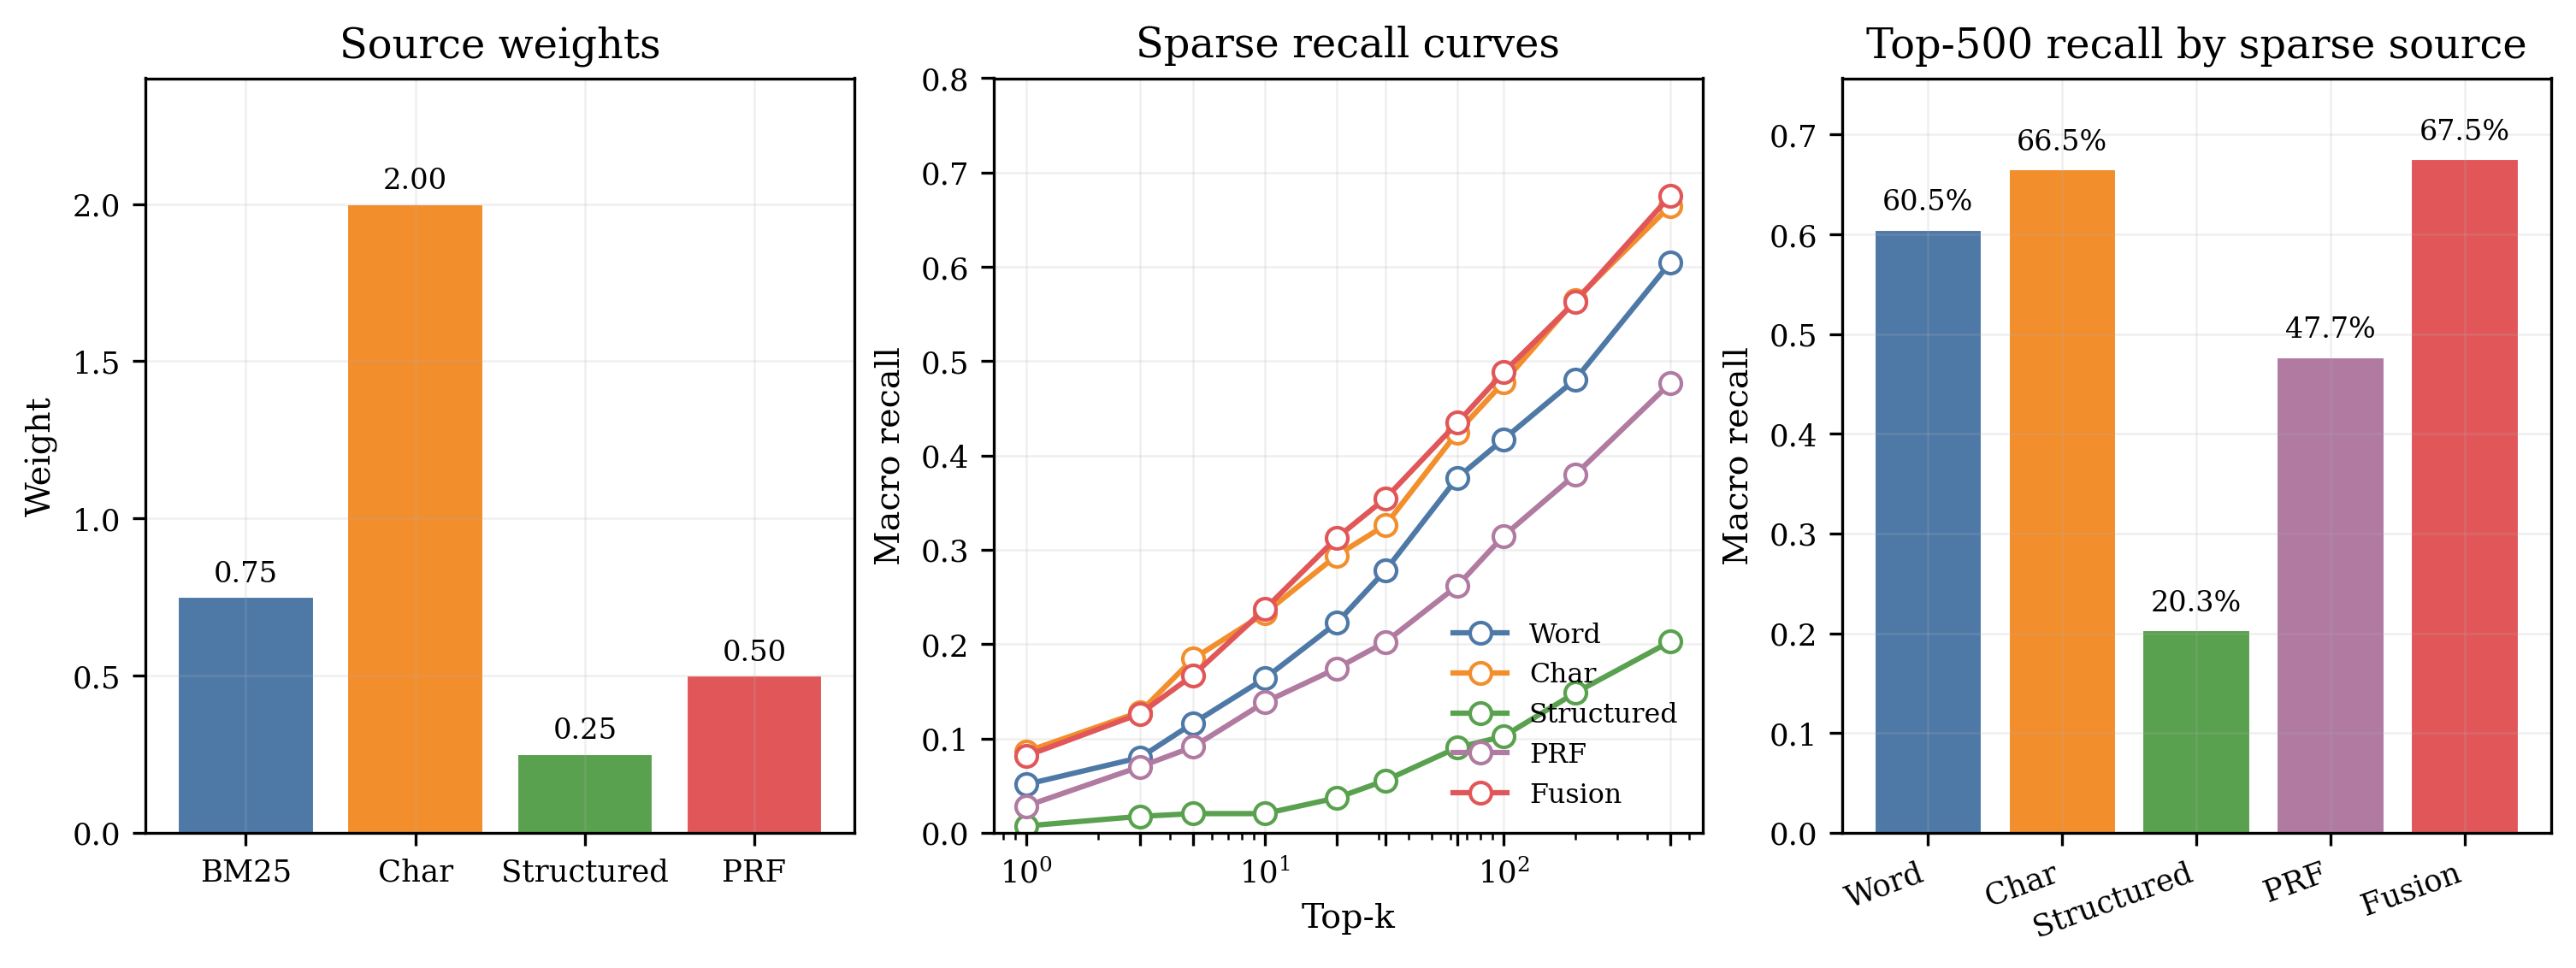
\includegraphics[width=0.96\textwidth]{figures/acl_sparse_multigate.png}
\caption{Sparse fusion gives the best top-500 recall and retains structured
cues for complementarity.  Character matching is the strongest single source;
structured cues improve fused recall under controlled ablation, so the final
system keeps a small structured weight.}
\label{fig:sparse}
\end{figure*}

Figures~\ref{fig:staging} and~\ref{fig:sparse} justify the candidate stage:
fusion improves top-500 recall over any single source, and staging concentrates
neural scoring on high-value candidate pools.

\subsection{Multi-Scale Feature Fusion}

Reranking fuses dense similarity, sparse source rank, word overlap, numeric
agreement, negation compatibility, and length shape.  MiniLM embeddings are
mean-pooled and $\ell_2$-normalized, following sentence-embedding retrieval
practice \citep{reimers2019sentence}, so cosine similarity is an inner product:
\[
s_{\mathrm{emb}}(c,d)=h(c)^\top h(d).
\]

The shallow factual features are summarized as
\[
\phi(c,d)=
[\phi_{\mathrm{rank}},\phi_{\mathrm{lex}},\phi_{\mathrm{num}},
\phi_{\mathrm{neg}},\phi_{\mathrm{len}},s_{\mathrm{emb}}].
\]
Here $\phi_{\mathrm{rank}}$ is the reciprocal sparse-source rank,
$\phi_{\mathrm{lex}}$ contains claim-normalized and evidence-normalized word
overlap, $\phi_{\mathrm{num}}$ counts shared numeric strings,
$\phi_{\mathrm{neg}}$ marks negation compatibility, and
$\phi_{\mathrm{len}}$ records normalized character-length difference.  A
lightweight gradient-boosted matcher is trained on gold claim--evidence pairs
and sampled non-gold candidates from the training claims.  It estimates
$p_{\mathrm{feat}}(c,d)$, the probability that a candidate is useful evidence
under these shallow signals.  The context score is
\[
S_{\mathrm{ctx}}(c,d)=
\alpha\,\widetilde{s}_{\mathrm{emb}}(c,d)
+(1-\alpha)\,p_{\mathrm{feat}}(c,d),
\]
where $\widetilde{s}_{\mathrm{emb}}$ is claim-wise normalized.  Embeddings handle
semantic relatedness; factual features guard against number, negation, and
lexical-grounding errors.

\begin{figure}[t]
\centering
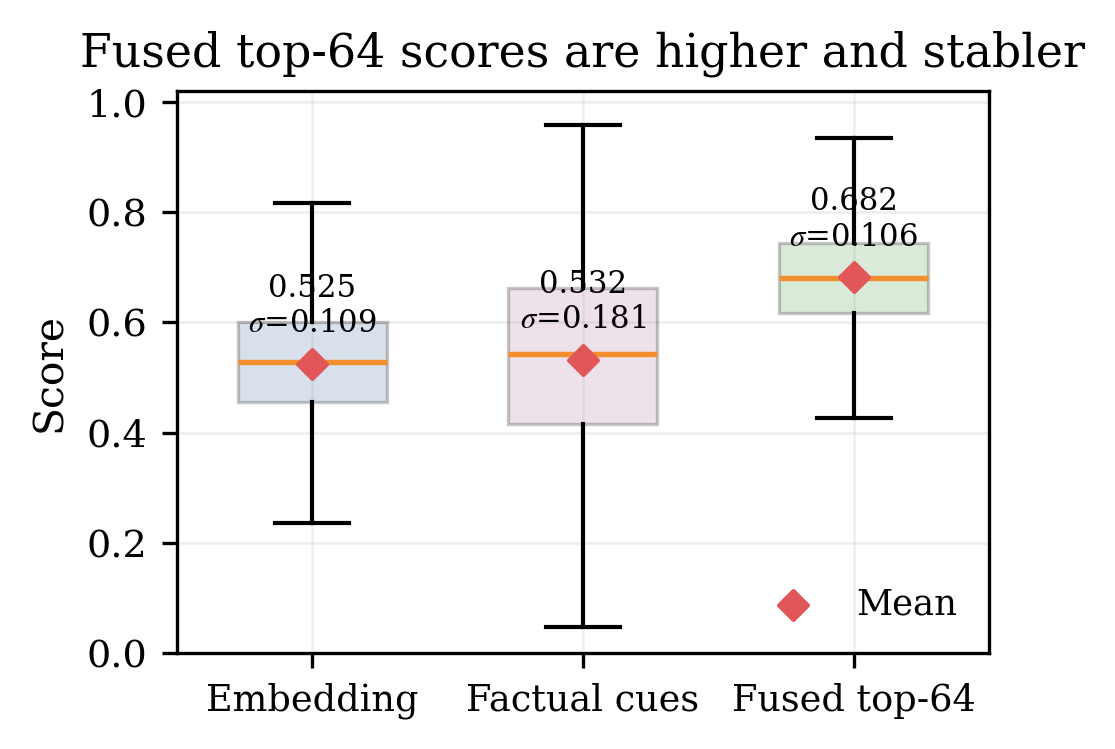
\includegraphics[width=\linewidth]{figures/acl_top64_score_distribution.png}
\caption{Top-64 fusion raises the retained-candidate score distribution and
reduces dispersion.  In the Colab diagnostic, fused scores have mean/std =
0.682/0.106, compared with 0.525/0.109 for embeddings and 0.532/0.181 for
factual cues.}
\label{fig:top64-score-distribution}
\end{figure}

\subsection{Bounded Neural Evidence Selection}

The submitted evidence stage uses a stricter operating point than the classifier
context.  Cross-encoders jointly encode claim and evidence
\citep{nogueira2019bert}, so we reserve them for the
sparse/embedding-prefiltered pool.  Candidate evidence text is truncated before
tokenization, then claim--evidence pairs are scored in PyTorch batches.
For each claim, raw cross-encoder logits and embedding similarities are
min--max normalized over the candidate pool.  The final evidence score fuses
cross-encoder confidence, embedding confidence, embedding rank, and sparse
source rank:
\[
\begin{aligned}
S_{\mathrm{sub}}(c,d)={}&
\beta_1\widetilde{s}_{\mathrm{CE}}
+\beta_2\widetilde{s}_{\mathrm{emb}}\\
&+\frac{\beta_3}{\tau+r_{\mathrm{emb}}}
+\frac{\beta_4}{\tau+r_{\mathrm{src}}}.
\end{aligned}
\]
Coefficients are fixed.  Candidates outside the cross-encoder subset remain
ranked by embedding and source-rank terms, which keeps neural cost bounded and
retains useful sparse candidates.

\begin{figure*}[t]
\centering
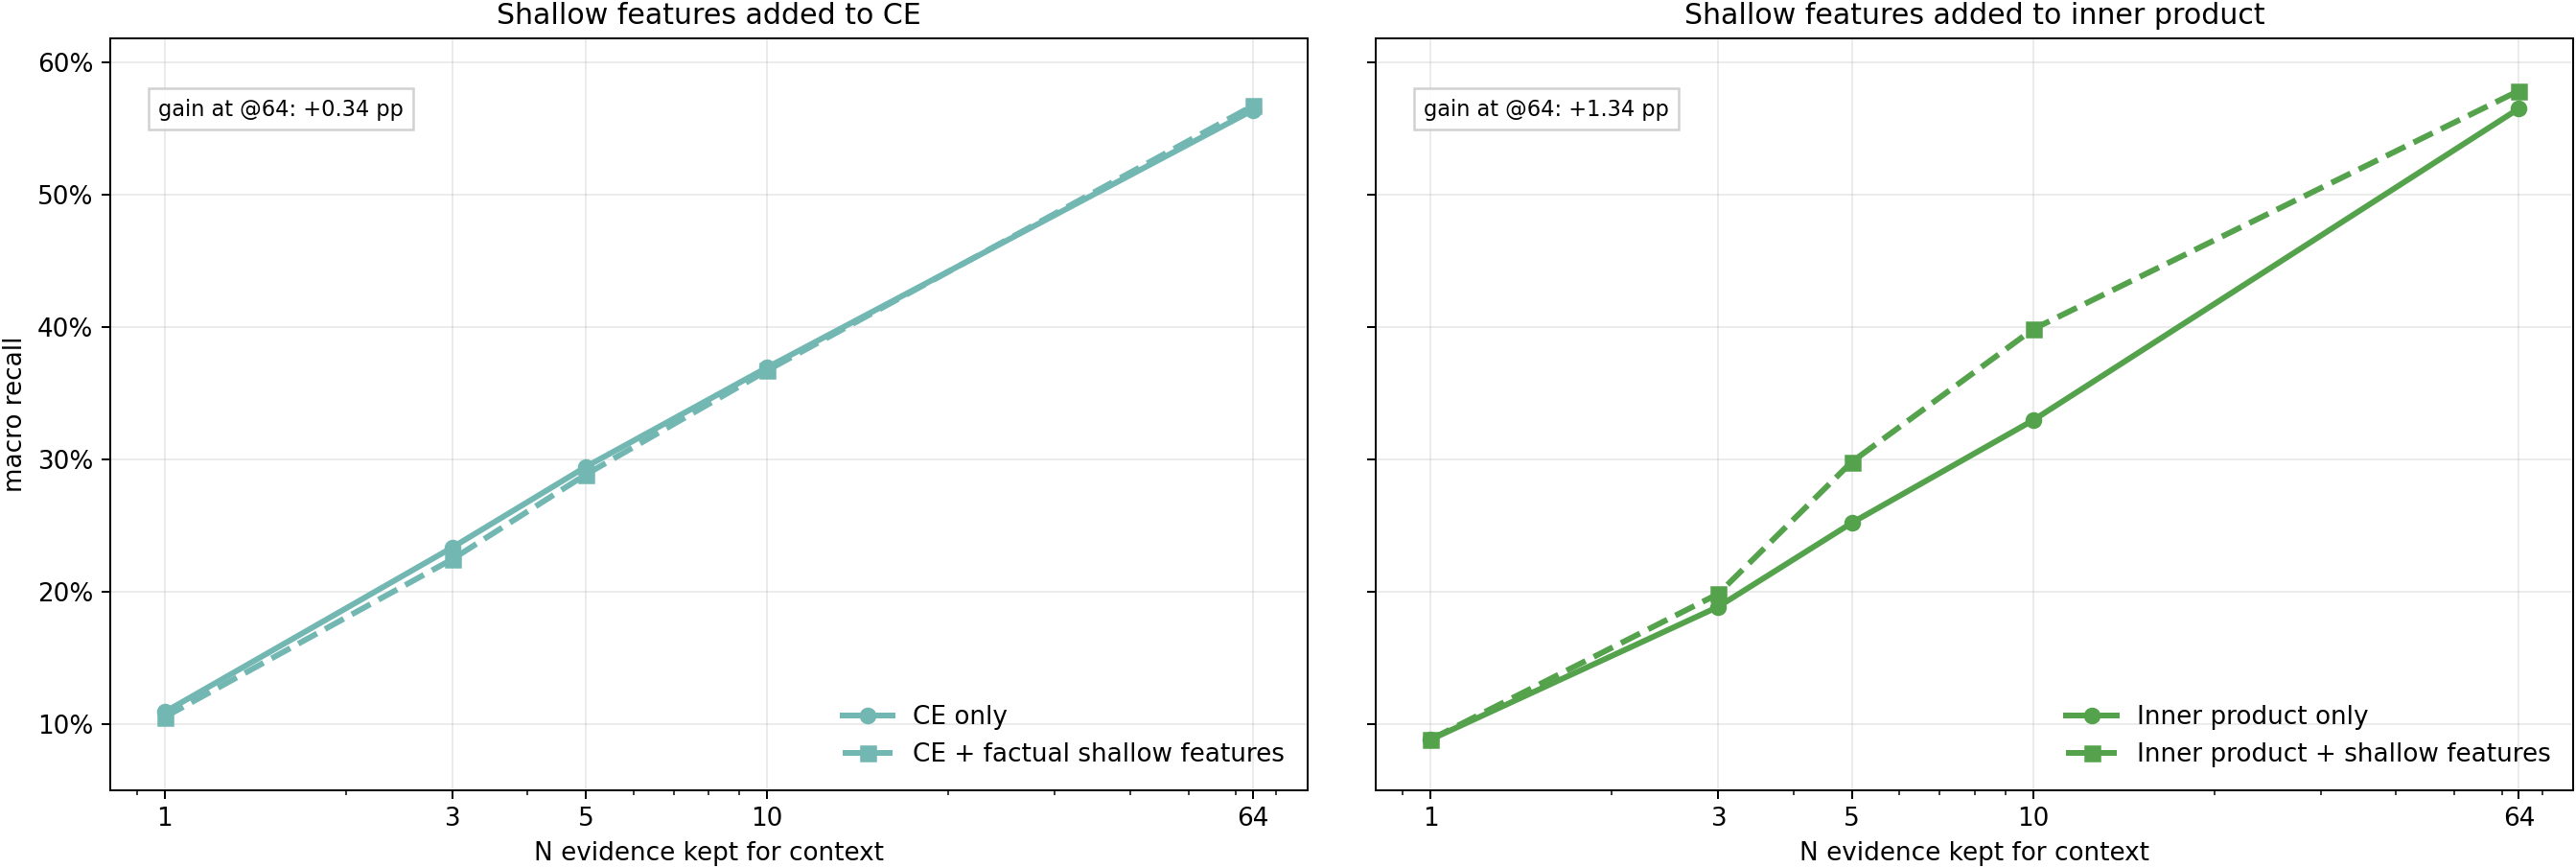
\includegraphics[width=0.96\textwidth]{figures/acl_shallow_complement.png}
\caption{Factual cues preserve or improve semantic ranking.  Cue gains are
larger for embedding inner product and smaller for the already strong
cross-encoder, supporting feature fusion over a purely semantic selector.}
\label{fig:shallow-complement}
\end{figure*}

Figures~\ref{fig:top64-selector}, \ref{fig:top64-score-distribution}, and
\ref{fig:shallow-complement} justify multi-scale fusion: factual cues act as
complementary signals that improve semantic ranking and stabilize the retained
candidate pool.

\subsection{Structured Evidence Classification}

The classifier predicts from a bounded ordered evidence context:
\[
x_c=[\mathrm{claim}; z_1,z_1,\ldots,z_m,z_m,z_{m+1},\ldots,z_L],
\]
where the highest-ranked evidence lines are repeated to raise their TF-IDF
weight.  The leading evidence receives a larger text budget, while later rows
are truncated so the context keeps more distinct evidence items.  Each evidence
line also gets a rank prefix plus cue tokens: a word-overlap bucket, number
match or mismatch status, claim-number-only status, and negation compatibility.
The logistic model learns weights for these cue tokens from training data.  Let
$v_c$ be the TF-IDF vector; a one-vs-rest logistic model learns one binary
classifier per label:
\[
P(y=k\mid c)=\sigma(\theta_k^\top v_c+b_k).
\]
The largest decision score gives the label.  This keeps classification cheap
while preserving retrieval rank and factual signals.

\FloatBarrier
\section{Results}

\subsection{Main Experimental Results}

The final system achieved an evidence retrieval F-score of 0.2021, claim
classification accuracy of 0.5000, a harmonic mean score of 0.2879, and a
classifier macro-F1 score of 0.4659, as shown in Table~\ref{tab:final}.
Overall, these results show that the system was able to balance retrieval
performance and classification accuracy while still remaining lightweight
enough to run within free Google Colab limitations. The sparse retrieval
experiments showed that combining multiple sparse retrieval methods improved
evidence recall compared to using only a single retrieval source.
Figure~\ref{fig:sparse} shows that the weighted reciprocal rank fusion
retriever achieved the highest top-500 macro recall of 67.5\%, outperforming
all individual sparse retrieval gates. Character-based retrieval achieved the
strongest standalone recall, while the structured retrieval gate still improved
the final fusion results by adding complementary factual information.

The staged retrieval pipeline also reduced computational cost while still
preserving useful evidence candidates. As shown in Table~\ref{tab:retrieval}
and Figure~\ref{fig:recall-vs-k}, recall gradually decreased as the candidate
pool became smaller across each retrieval stage. The sparse top-500 stage
achieved 67.5\% macro recall, while the reranked top-64 context pool retained
57.8\% macro recall. After the final top-3 evidence selection stage, the
submitted evidence set achieved an evidence retrieval F-score of 0.2021. The
reranking experiments further showed that combining semantic embeddings with
shallow factual cues improved evidence selection quality.
Figure~\ref{fig:top64-selector} shows that the embedding-plus-cues selector
achieved the highest top-64 macro recall of 57.8\%, outperforming both the
sparse cutoff baseline and the cross-encoder-plus-cues configuration.
Figure~\ref{fig:top64-score-distribution} also shows that the fused retrieval
scores produced a more stable retained candidate distribution compared to using
embeddings or factual cues alone. The classifier diagnostics in
Figure~\ref{fig:final-classifier} show that the model performed best on the
SUPPORTS class, while most classification errors occurred between SUPPORTS,
REFUTES and NOT-ENOUGH-INFO. The DISPUTED class was the hardest class to
classify due to the smaller number of development examples and more ambiguous
evidence relationships.

\subsection{Ablation Study}

The ablation experiments showed that both factual feature fusion and structured
evidence formatting improved downstream classification performance.
Figure~\ref{fig:shallow-complement} shows that adding shallow factual cues
consistently improved semantic ranking performance for both embedding
similarity and cross-encoder retrieval. The improvements were more noticeable
for embedding similarity, suggesting that lexical overlap, number agreement and
negation matching helped preserve stronger factual consistency between claims
and evidence. The classifier ablation experiments in
Table~\ref{tab:classifier-ablation} also showed that structured evidence
formatting performed better than plain evidence concatenation. The plain
context representation achieved an accuracy of 0.4351 and macro-F1 score of
0.3762, while the enhanced context representation improved performance to
0.4935 accuracy and 0.4544 macro-F1 at C = 0.25. The best overall development
performance was achieved using the enhanced representation with C = 0.125,
reaching 0.5195 accuracy and 0.4841 macro-F1.

\subsection{Sensitivity Analysis}

The retrieval sensitivity analysis showed that evidence recall was highly
dependent on the retained evidence budget. Figure~\ref{fig:recall-vs-k} shows
that retrieval recall gradually decreased as fewer evidence candidates were
retained. However, the staged retrieval architecture was still able to preserve
most recoverable evidence while significantly reducing the number of
claim-evidence pairs requiring neural scoring. The classifier sensitivity
analysis in Table~\ref{tab:classifier-ablation} showed that logistic regression
regularisation strength affected classification performance. Lower C values
achieved stronger generalisation performance, with the best macro-F1 score
achieved at C = 0.125. Performance gradually decreased as C increased,
suggesting that stronger regularisation helped reduce overfitting within the
structured evidence representation.


\begin{table}[t]
\centering
\small
\begin{tabular}{lrrr}
\toprule
Stage & F-score & Macro recall & Hit-any \\
\midrule
Sparse top-500 & 0.0083 & 0.6754 & 0.9026 \\
Context top-64 & 0.0517 & 0.5784 & 0.8636 \\
Submitted top-3 & 0.2021 & 0.2355 & 0.4675 \\
\bottomrule
\end{tabular}
\caption{Retrieval metrics from the self-generated notebook artifacts.}
\label{tab:retrieval}
\end{table}

\begin{figure}[t]
\centering
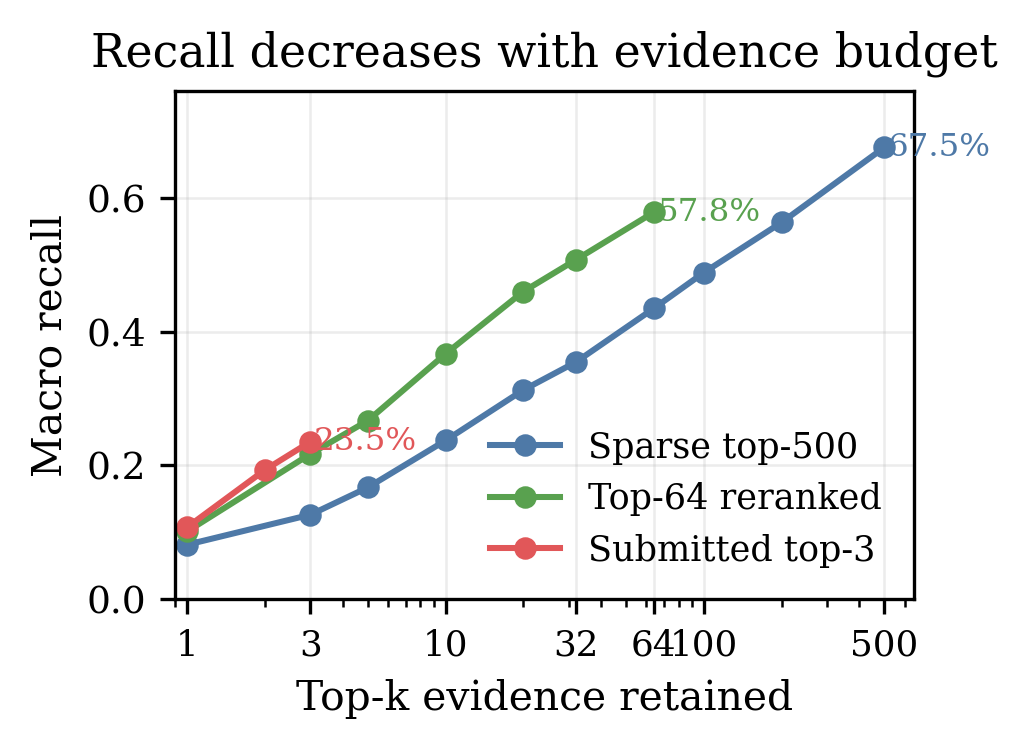
\includegraphics[width=\linewidth]{figures/acl_recall_vs_k.png}
\caption{Recall-vs-K curves show the pruning trade-off behind the selected
operating points.  The sparse pool keeps broad top-500 recall, the reranked
pool preserves most recoverable evidence at top-64, and the submitted top-3 is
the strict evidence set used for scoring.}
\label{fig:recall-vs-k}
\end{figure}

\begin{table}[t]
\centering
\small
\begin{tabular}{lr}
\toprule
Metric & Value \\
\midrule
Evidence Retrieval F-score ($F$) & 0.2021 \\
Claim Classification Accuracy ($A$) & 0.5000 \\
Harmonic Mean of $F$ and $A$ ($H$) & 0.2879 \\
Top-3 Macro Recall & 0.2355 \\
Classifier Macro-F1 & 0.4659 \\
\bottomrule
\end{tabular}
\caption{Final Colab-reproduced development result.  $F$, $A$, and
$H=2FA/(F+A)$ are official course metrics; the last two rows summarize retrieval
and classification behavior.}
\label{tab:final}
\end{table}

\begin{figure*}[t]
\centering

\includegraphics[width=0.84\textwidth]{figures/acl_classifier_summary.png}
\caption{Classifier diagnostics.  Row-normalized confusion controls for class
support, and per-class precision/recall/F1 summarizes the classification
report.}
\label{fig:final-classifier}
\end{figure*}

\begin{table*}[t]
\centering
\scriptsize
\renewcommand{\arraystretch}{0.88}
\begin{minipage}[t]{0.62\textwidth}
\centering
\begin{tabular}{lrrr}
\toprule
Evidence input variant & $C$ & Acc. & Macro-F1 \\
\midrule
Plain evidence text & 0.25 & 0.4351 & 0.3762 \\
Add evidence rank token & 0.25 & 0.4351 & 0.3749 \\
Repeat top evidence & 0.25 & 0.4416 & 0.3938 \\
Rank-weighted text budget & 0.25 & 0.4351 & 0.3882 \\
Add factual cue tokens & 0.25 & 0.4935 & 0.4544 \\
Factual cues + tuned $C$ & 0.125 & 0.5195 & 0.4841 \\
\bottomrule
\end{tabular}
\end{minipage}
\hfill
\begin{minipage}[t]{0.32\textwidth}
\centering
\begin{tabular}{rrr}
\toprule
LogReg $C$ & Acc. & Macro-F1 \\
\midrule
0.125 & 0.5195 & 0.4841 \\
0.25 & 0.4935 & 0.4544 \\
0.5 & 0.4740 & 0.4263 \\
1.0 & 0.4675 & 0.4184 \\
2.0 & 0.4416 & 0.3825 \\
4.0 & 0.4545 & 0.3913 \\
8.0 & 0.4481 & 0.3925 \\
\bottomrule
\end{tabular}
\end{minipage}
\caption{Classifier ablations.  The left block compares how retrieved evidence
is formatted before TF-IDF classification.  The right block keeps the factual
cue format fixed and sweeps logistic-regression regularization.}
\label{tab:classifier-ablation}
\end{table*}

\section{Discussion and Critical Analysis}

The results showed that evidence retrieval quality had a major impact on
overall performance. Better retrieval generally led to stronger classification
because the classifier relied on receiving relevant evidence. The staged
retrieval architecture therefore worked well for the resource-constrained
setting: it preserved useful candidates while reducing the pool before applying
more expensive neural reranking.

Sparse retrieval remained important even when semantic reranking was used later.
Character-based retrieval was especially strong because climate claims often
contain scientific terminology, abbreviations, and numeric expressions that
benefit from partial lexical matching. Reciprocal rank fusion improved recall
by combining complementary sparse evidence relationships. The reranking
experiments also showed that semantic similarity alone was not enough: shallow
factual cues such as lexical overlap, number agreement, and negation matching
helped preserve factual consistency between claims and evidence.

The classifier ablations showed the same pattern downstream. Enhanced evidence
formatting preserved rank information and factual cue tokens, allowing the
TF-IDF logistic regression classifier to learn stronger patterns than plain
concatenation. The main limitation is still evidence selection: exact gold
evidence retrieval remains difficult, and the DISPUTED class is hard because it
has fewer examples and requires reasoning over more ambiguous evidence
relationships.

\section{Conclusion}
\enlargethispage{4\baselineskip}

This paper examined how to balance claim-label accuracy, evidence recall, and
runtime for climate claim fact-checking under free Google Colab constraints.
The final pipeline combines multi-gate sparse retrieval, feature-fusion
reranking, bounded cross-encoder evidence selection, and structured TF-IDF
classification. On the development set, it achieved evidence F-score 0.2021,
claim accuracy 0.5000, harmonic mean 0.2879, and classifier macro-F1 0.4659.

The main conclusion is that retrieval signals should be carried forward rather
than discarded. Multi-gate sparse fusion reached 67.5\% macro recall at top-500,
shallow factual cues improved semantic reranking, and structured evidence input
improved classification over plain concatenation. The remaining bottleneck is
top-3 selection, where many exact gold passages are still lost before final
submission, especially for DISPUTED claims.

\paragraph{Team contributions.}
Kaitlyn worked on results, discussion, introduction, and code. Jun worked on
imagery, introduction, references, method, and code. Om worked on the abstract,
related work, conclusion, references, and code.

\begingroup
\small
\setlength{\bibsep}{0pt}
\bibliography{custom}
\endgroup

\end{document}
